\documentclass{article}

\usepackage[spanish,activeacute]{babel}
\usepackage{amsfonts}
\usepackage{graphicx}
\usepackage{whilecode2}


\title{Taller 1}
\author{Mónica López Pola}

\begin{document}

\maketitle

\section*{Actividad 1}
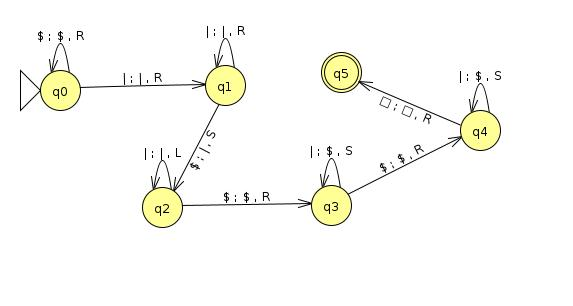
\includegraphics[scale=0.75]{MT3-4}

\section*{Apartado 2}
\begin{equation}
suma3 = <<\pi^1_1|\sigma(\pi^3_3)>|\sigma(\pi^4_4)>
\end{equation}
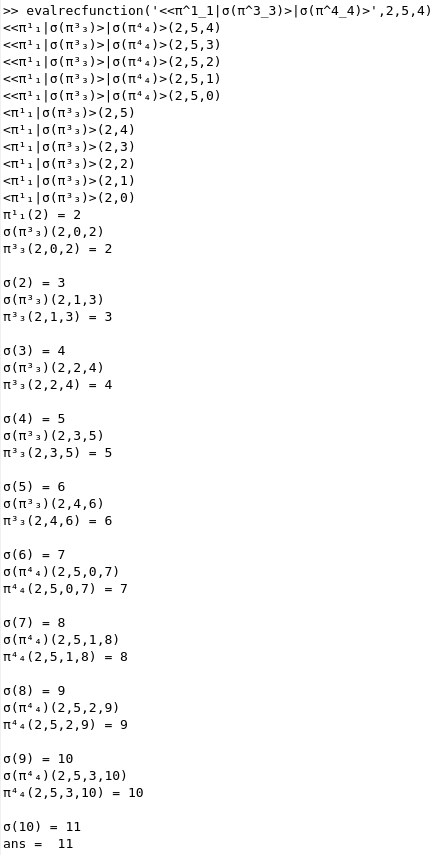
\includegraphics[scale=0.5]{funcion}

\section*{Apartado 3}
\begin{whilecode}[H]
$X_4 \Assig 0$

 \While{$X_1 \not = 0$}{

  $X_1 \Assig X_1 - 1$\;
  $X_4 \Assig X_4 + 1$

 }
 
  \While{$X_2 \not = 0$}{

  $X_2 \Assig X_2 - 1$\;
  $X_4 \Assig X_4 + 1$

 }
 
  \While{$X_3 \not = 0$}{

  $X_3 \Assig X_3 - 1$\;
  $X_4 \Assig X_4 + 1$

 }
 
 $X_1 \Assig X_4$
 \end{whilecode}

\end{document}